% Copyright (C) 2013 - Michael Baudin
%
% This file must be used under the terms of the 
% Creative Commons Attribution-ShareAlike 3.0 Unported License :
% http://creativecommons.org/licenses/by-sa/3.0/

    \chapter{Gallery}

The goal of this section is to gather experiments showing 
	  2D pictures of low disrepancy sequences.

%%%%%%%%%%%%%%%%%%%%%%%%%%%%%%%%%%%%%%%%%%%%%%%%%%%%%%%%%%%
\section{Van Der Corput Sequence}

      The Van Der Corput base 2 sequence is just the first dimension of 
	  the Halton sequence in 1 dimension. 
	  In the following script, we generate 15 points from the 
	  Halton sequence in 1 dimension.

\lstset{language=scilabscript}
\begin{lstlisting}
u=lowdisc_ldgen(15,1,"halton")
\end{lstlisting}

      The previous script produces the following output.

\lstset{language=scilabscript}
\begin{lstlisting}
-->u=lowdisc_ldgen(15,1,"halton")
 u  =
    0.5     
    0.25    
    0.75    
    0.125   
    0.625   
    0.375   
    0.875   
    0.0625  
    0.5625  
    0.3125  
    0.8125  
    0.1875  
    0.6875  
    0.4375  
    0.9375  
\end{lstlisting}

    
      We notice that the values are organized block by block, 
	  where the size of a block is a power of two. 
	  The block \#1 has x=0.5 (1 point). 
	  The block \#2 has x=0.25 and x=0.75 (2 points). 
	  The block \#3 has x=0.125 to x=0.875 (4 points). 
	  This is consistent with the fact that the Van Der Corput 
	  sequence that we consider here has base 2.
    

    
      In order to understand how this sequence fills the interval [0,1], 
	  we analyze the elements of the sequence in more detail. 
	  The following function prints each element of the sequence, 
	  by decomposing the number $n=u 2^p$, where u is the low discrepancy 
	  number and p is an appropriate integer. 
	  This allows to get the binary decomposition of the number u.
    

\lstset{language=scilabscript}
\begin{lstlisting}
function printVDC(u,p)
    nrows=size(u,"r")
    for i=1:nrows
        n=u(i)*2^p;
        d=number_tobary(n,[],[],p);
        s=strcat(string(d'),"");
        mprintf("u=%f, n=%3d, binary=0.%s\n",u(i),n,s)
    end
endfunction
\end{lstlisting}

    
      The following script computes the elements of the Van Der Corput 
	  sequence, block by block: 
	  we get the first point, then two more points, then 4 points, 
	  and finally 8 points.
    

\lstset{language=scilabscript}
\begin{lstlisting}
lds = lowdisc_new("halton");
lds = lowdisc_configure(lds,"-dimension",1);
lds = lowdisc_startup (lds);
[lds,u]=lowdisc_next(lds,1);
printVDC(u,1)
[lds,u]=lowdisc_next(lds,2);
printVDC(u,2)
[lds,u]=lowdisc_next(lds,4);
printVDC(u,3)
[lds,u]=lowdisc_next(lds,8);
printVDC(u,4)
lds = lowdisc_destroy (lds);
\end{lstlisting}

    
      The previous script produces the following output.
	  For example, $u=0.5625$ is decomposed in base-2 as 0.1001, 
	  since $0.5625=1/2+1/2^4$.
    

\lstset{language=scilabscript}
\begin{lstlisting}
u=0.500000, n=  1, binary=0.1
u=0.250000, n=  1, binary=0.01
u=0.750000, n=  3, binary=0.11
u=0.125000, n=  1, binary=0.001
u=0.625000, n=  5, binary=0.101
u=0.375000, n=  3, binary=0.011
u=0.875000, n=  7, binary=0.111
u=0.062500, n=  1, binary=0.0001
u=0.562500, n=  9, binary=0.1001
u=0.312500, n=  5, binary=0.0101
u=0.812500, n= 13, binary=0.1101
u=0.187500, n=  3, binary=0.0011
u=0.687500, n= 11, binary=0.1011
u=0.437500, n=  7, binary=0.0111
u=0.937500, n= 15, binary=0.1111
\end{lstlisting}

    
      Notice that the most significant digit (the 0 or 1 just after the 
	  decimal point) is alternatively 0, 1, 0, etc... 
	  Hence, the point altenates below and over the central value x=0.5.
    

    
      In order to see where the points are located in the interval [0,1], 
	  we plot the points block-by-block, where the y-coordinate corresponds 
	  to the index of the block.
    
	
\lstset{language=scilabscript}
\begin{lstlisting}
scf();
lds = lowdisc_new("halton");
lds = lowdisc_configure(lds,"-dimension",1);
lds = lowdisc_startup (lds);
k=1;
imax=5;
for i=1:5
    npoints=2^(i-1);
    [lds,u]=lowdisc_next(lds,npoints);
    plot(u',i,"bo")
    xstring(u',i,string(k:k+npoints-1))
    k=k+npoints;
end
lds = lowdisc_destroy (lds);
a = gca();
a.data_bounds=[
0 0
1 imax+1
];
xtitle("Van Der Corput Sequence (base 2)",..
"X","Block Index")
\end{lstlisting}

    
      The previous script produces the figure \ref{fig-vdcb2}.
    

\begin{figure}[htbp]
\begin{center}
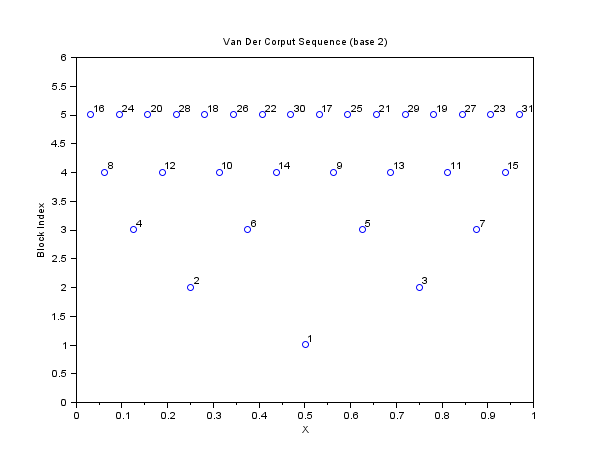
\includegraphics[width=15cm]{figures/vandercorput-base2.png}
\end{center}
\caption{The Van Der Corput sequence in base 2.}
\label{fig-vdcb2}
\end{figure}
	
    
      We see that each block fills the interval with regular spacings, 
	  but that the order of the points is so that 
	  two consecutive points in the sequence always have x=0.5 in-between.
    

%%%%%%%%%%%%%%%%%%%%%%%%%%%%%%%%%%%%%%%%%%%%%%%%%%%%%%%%%%%
\section{Halton Sequence}

\lstset{language=scilabscript}
\begin{lstlisting}
u=lowdisc_ldgen ( 1000 , 2 , "halton" );
scf(); 
plot(u(:,1),u(:,2),"bo")
xtitle("Halton: 1000 points","X1","X2")
\end{lstlisting}

    
      The previous script produces the figure \ref{fig-haltons2n1000}.
    
\begin{figure}[htbp]
\begin{center}
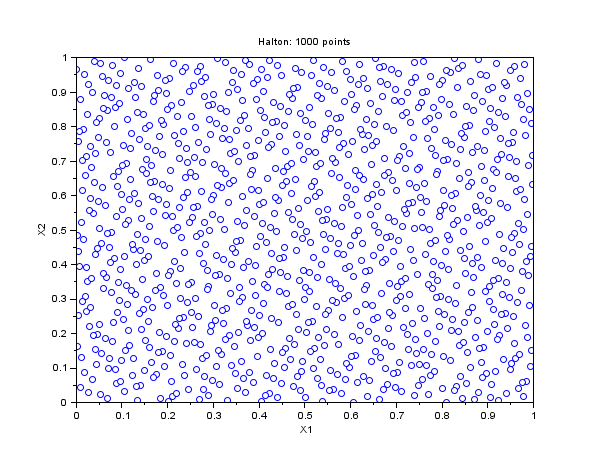
\includegraphics[width=15cm]{figures/halton-s2-n1000.png}
\end{center}
\caption{The Halton sequence - 1000 points in 2 dimensions.}
\label{fig-haltons2n1000}
\end{figure}

%%%%%%%%%%%%%%%%%%%%%%%%%%%%%%%%%%%%%%%%%%%%%%%%%%%%%%%%%%%
\section{Scrambled (RR2) Halton Sequence}

	
      The following script produces a scrambled Halton sequence, 
	  with the permutation of Kocis and Whiten (RR2).
    

\lstset{language=scilabscript}
\begin{lstlisting}
u=lowdisc_ldgen ( 1000 , 2 , "halton-scrambled" );
scf(); 
plot(u(:,1),u(:,2),"bo")
xtitle("Scrambled Halton: 1000 points","X1","X2")
\end{lstlisting}

    
      The previous script produces the figure \ref{fig-halton-RR2-s2-n1000}.
    
\begin{figure}[htbp]
\begin{center}
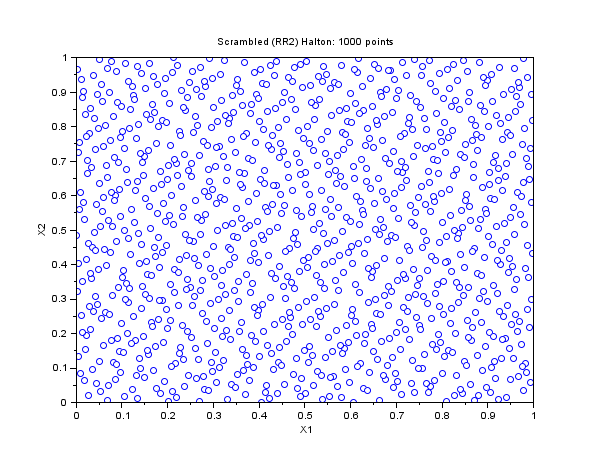
\includegraphics[width=15cm]{figures/halton-RR2-s2-n1000.png}
\end{center}
\caption{The scrambled Halton-RR2 sequence - 1000 points in 2 dimensions.}
\label{fig-halton-RR2-s2-n1000}
\end{figure}

%%%%%%%%%%%%%%%%%%%%%%%%%%%%%%%%%%%%%%%%%%%%%%%%%%%%%%%%%%%
\section{Leaped Halton Sequence}

	
      The following script produces a leaped Halton sequence. 
	  The leap parameter is automatically computed by the \scifun{lowdisc\_haltonsuggest} 
	  function. 
    

\lstset{language=scilabscript}
\begin{lstlisting}
u=lowdisc_ldgen ( 1000 , 2 , "halton-leaped" );
scf(); 
plot(u(:,1),u(:,2),"bo")
xtitle("Leaped Halton: 1000 points","X1","X2")
\end{lstlisting}

    
      The previous script produces the figure \ref{fig-halton-leaped-s2-n1000}.
    
\begin{figure}[htbp]
\begin{center}
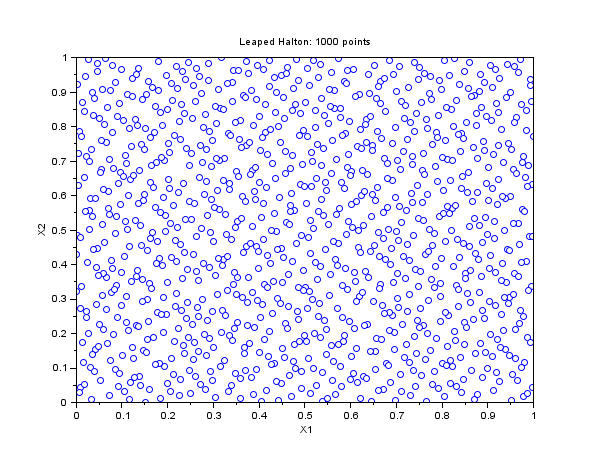
\includegraphics[width=15cm]{figures/halton-leaped-s2-n1000.png}
\end{center}
\caption{The Halton leaped sequence - 1000 points in 2 dimensions.}
\label{fig-halton-leaped-s2-n1000}
\end{figure}


    
%%%%%%%%%%%%%%%%%%%%%%%%%%%%%%%%%%%%%%%%%%%%%%%%%%%%%%%%%%%
\section{Reverse-Halton Sequence}

\lstset{language=scilabscript}
\begin{lstlisting}
u=lowdisc_ldgen ( 1000 , 2 , "halton-reverse" );
scf(); 
plot(u(:,1),u(:,2),"bo")
xtitle("Reverse-Halton: 1000 points","X1","X2")
\end{lstlisting}

    
      The previous script produces the figure \ref{fig-reversehalton-s2-n1000}.
    
\begin{figure}[htbp]
\begin{center}
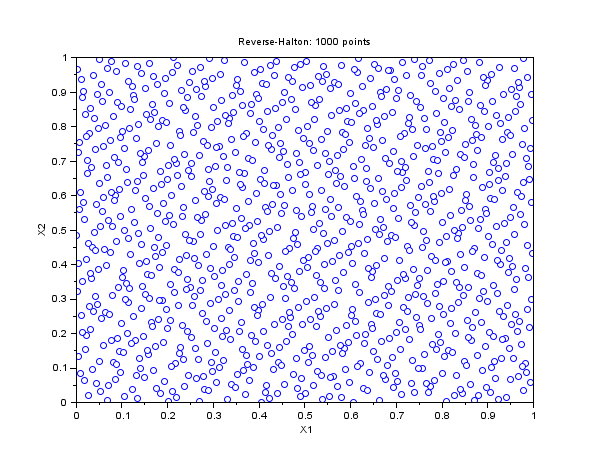
\includegraphics[width=15cm]{figures/reversehalton-s2-n1000.png}
\end{center}
\caption{The Reverse Halton sequence - 1000 points in 2 dimensions.}
\label{fig-reversehalton-s2-n1000}
\end{figure}


    
%%%%%%%%%%%%%%%%%%%%%%%%%%%%%%%%%%%%%%%%%%%%%%%%%%%%%%%%%%%
\section{Sobol Sequence}

\lstset{language=scilabscript}
\begin{lstlisting}
u=lowdisc_ldgen ( 1000 , 2 , "sobol" );
scf(); 
plot(u(:,1),u(:,2),"bo")
xtitle("Sobol: 1000 points","X1","X2")
\end{lstlisting}

    
      The previous script produces the figure \ref{fig-sobol-s2-n1000}.
    
\begin{figure}[htbp]
\begin{center}
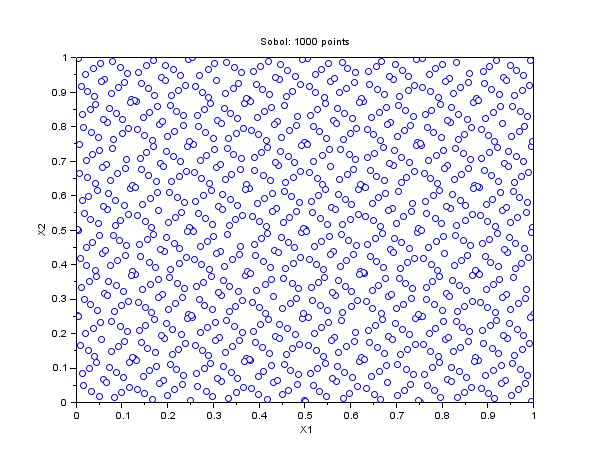
\includegraphics[width=15cm]{figures/sobol-s2-n1000.png}
\end{center}
\caption{The Sobol sequence - 1000 points in 2 dimensions.}
\label{fig-sobol-s2-n1000}
\end{figure}

    
%%%%%%%%%%%%%%%%%%%%%%%%%%%%%%%%%%%%%%%%%%%%%%%%%%%%%%%%%%%
\section{Faure Sequence}

\lstset{language=scilabscript}
\begin{lstlisting}
u=lowdisc_ldgen ( 1000 , 2 , "faure" );
scf(); 
plot(u(:,1),u(:,2),"bo")
xtitle("Faure: 1000 points","X1","X2")
\end{lstlisting}

    
      The previous script produces the figure \ref{fig-faure-s2-n1000}.
    
\begin{figure}[htbp]
\begin{center}
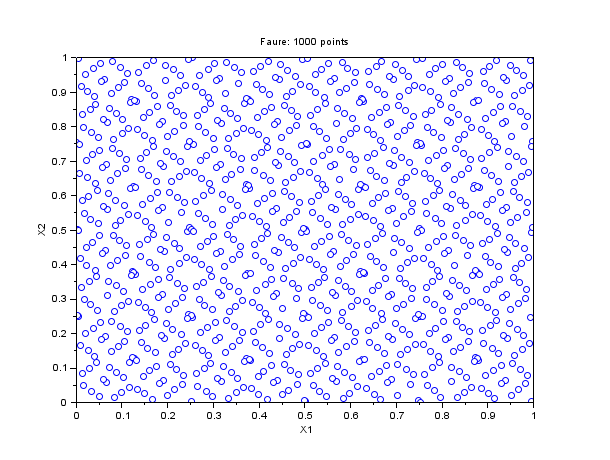
\includegraphics[width=15cm]{figures/faure-s2-n1000.png}
\end{center}
\caption{The Faure sequence - 1000 points in 2 dimensions.}
\label{fig-faure-s2-n1000}
\end{figure}

    
%%%%%%%%%%%%%%%%%%%%%%%%%%%%%%%%%%%%%%%%%%%%%%%%%%%%%%%%%%%
\section{Niederreiter Sequence}

\lstset{language=scilabscript}
\begin{lstlisting}
u=lowdisc_ldgen ( 1000 , 2 , "niederreiter" );
scf(); 
plot(u(:,1),u(:,2),"bo")
xtitle("Niederreiter: 1000 points","X1","X2")
\end{lstlisting}

    
      The previous script produces the figure \ref{fig-niederreiter-s2-n100}.
    
\begin{figure}[htbp]
\begin{center}
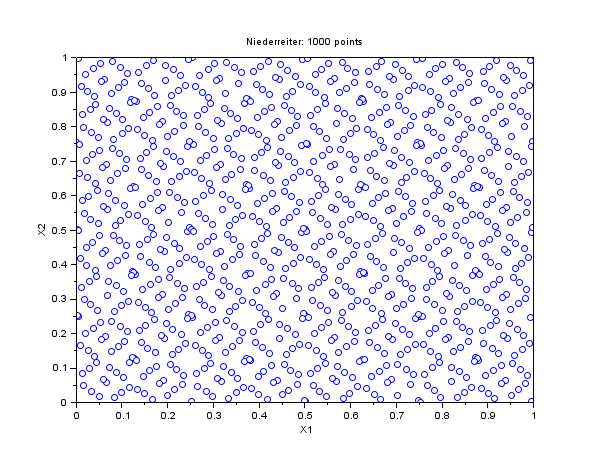
\includegraphics[width=15cm]{figures/niederreiter-s2-n1000.png}
\end{center}
\caption{The Niederreiter sequence in base 2 - 1000 points in 2 dimensions.}
\label{fig-niederreiter-s2-n100}
\end{figure}


    
%%%%%%%%%%%%%%%%%%%%%%%%%%%%%%%%%%%%%%%%%%%%%%%%%%%%%%%%%%%
\section{Scrambled Sobol Sequence}

\lstset{language=scilabscript}
\begin{lstlisting}
//
// No Scrambling
//
lds=lowdisc_new("sobol");
lds=lowdisc_configure(lds,"-dimension",2);
lds = lowdisc_startup (lds);
[lds,u] = lowdisc_next (lds,100);
lds=lowdisc_destroy(lds);
//
// Owen Scrambling
//
lds=lowdisc_new("sobol");
lds=lowdisc_configure(lds,"-dimension",2);
lds=lowdisc_configure(lds,"-scrambling","Owen");
lds = lowdisc_startup (lds);
[lds,uO] = lowdisc_next (lds,100);
lds=lowdisc_destroy(lds);
//
// Faure-Tezuka Scrambling
//
lds=lowdisc_new("sobol");
lds=lowdisc_configure(lds,"-dimension",2);
lds=lowdisc_configure(lds,"-scrambling","Faure-Tezuka");
lds = lowdisc_startup (lds);
[lds,uFT] = lowdisc_next (lds,100);
lds=lowdisc_destroy(lds);
//
// Owen-Faure-Tezuka Scrambling
//
lds=lowdisc_new("sobol");
lds=lowdisc_configure(lds,"-dimension",2);
lds=lowdisc_configure(lds,"-scrambling","Owen-Faure-Tezuka");
lds = lowdisc_startup (lds);
[lds,uOFT] = lowdisc_next (lds,100);
lds=lowdisc_destroy(lds);
//
// Make a plot
//
scf();
subplot(2,2,1);
plot(u(:,1),u(:,2),"b.");
xtitle("Sobol","X1","X2");
subplot(2,2,2);
plot(uO(:,1),uO(:,2),"b.");
xtitle("Owen Scrambled Sobol","X1","X2");
subplot(2,2,3);
plot(uFT(:,1),uFT(:,2),"b.");
xtitle("Faure-Tezuka Scrambled Sobol","X1","X2");
subplot(2,2,4);
plot(uOFT(:,1),uOFT(:,2),"b.");
xtitle("Owen-Faure-Tezuka Scrambled Sobol","X1","X2");
\end{lstlisting}

    
      The previous script produces the figure \ref{fig-sobol-scrambled-s2-n100}.
    
\begin{figure}[htbp]
\begin{center}
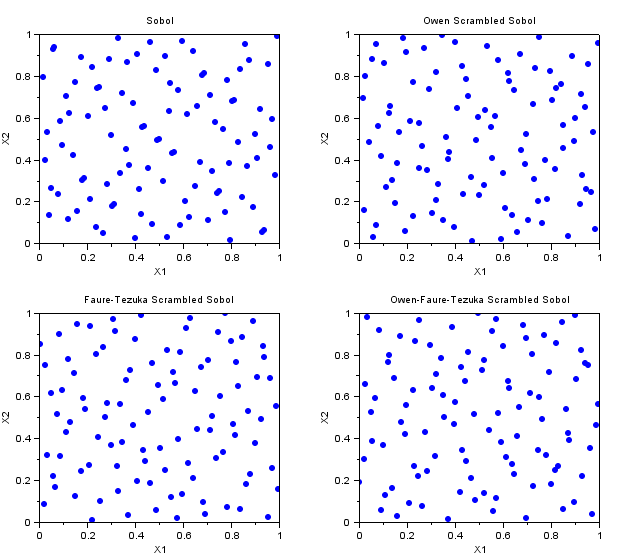
\includegraphics[width=15cm]{figures/sobol-scrambled-s2-n100.png}
\end{center}
\caption{The scrambled Sobol sequence 100 points in 2 dimensions.}
\label{fig-sobol-scrambled-s2-n100}
\end{figure}

    
%%%%%%%%%%%%%%%%%%%%%%%%%%%%%%%%%%%%%%%%%%%%%%%%%%%%%%%%%%%
\section{Note on 2D plots}
	
	  As we have seen, in 2D the Sobol, Niederreiter (base 2) and 
	  Faure sequences are essentially the same. 
	

	\lstset{language=scilabscript}
\begin{lstlisting}
i=(1:2^4-1)';
u1=lowdisc_ldgen ( 2^4-1 , 2 , "sobol" );
u2=lowdisc_ldgen ( 2^4-1 , 2 , "faure" );
u3=lowdisc_ldgen ( 2^4-1 , 2 , "niederreiter" );
disp([i,u1,u2,u3])
\end{lstlisting}

\lstset{language=scilabscript}
\begin{lstlisting}
           Sobol              Faure              Niederreiter        
    n      X1        X2       X1        X2       X1        X2        
    1.     0.5       0.5      0.5       0.5      0.5       0.5       
    2.     0.75      0.25     0.25      0.75     0.25      0.75      
    3.     0.25      0.75     0.75      0.25     0.75      0.25      
    4.     0.375     0.375    0.125     0.625    0.125     0.625     
    5.     0.875     0.875    0.625     0.125    0.625     0.125     
    6.     0.625     0.125    0.375     0.375    0.375     0.375     
    7.     0.125     0.625    0.875     0.875    0.875     0.875     
    8.     0.1875    0.3125   0.0625    0.9375   0.0625    0.9375    
    9.     0.6875    0.8125   0.5625    0.4375   0.5625    0.4375    
    10.    0.9375    0.0625   0.3125    0.1875   0.3125    0.1875    
    11.    0.4375    0.5625   0.8125    0.6875   0.8125    0.6875    
    12.    0.3125    0.1875   0.1875    0.3125   0.1875    0.3125    
    13.    0.8125    0.6875   0.6875    0.8125   0.6875    0.8125    
    14.    0.5625    0.4375   0.4375    0.5625   0.4375    0.5625    
    15.    0.0625    0.9375   0.9375    0.0625   0.9375    0.0625    
\end{lstlisting}
	
	  The points are coming by blocks which size is a power of 2. 
	  A part of the reason is because all these sequences 
	  in two dimensions are based on the first prime, which is 2.
	
	
	  The Niederreiter (base 2) and Faure sequences produce 
	  exactly the same points, in the same order. 
	  The Sobol points are also the same, but come in a different order. 
	  For example, the point n=15 in Sobol sequence 
	  is the same as point n=8 in Niederreiter (base 2) sequence.
	
%%%%%%%%%%%%%%%%%%%%%%%%%%%%%%%%%%%%%%%%%%%%%%%%%%%%%%%%%%%
\section{In 3D}

	
	  Since the 2D Niederreiter, Sobol and Faure sequences are the same, 
	  we consider 3D sequences.
	

\lstset{language=scilabscript}
\begin{lstlisting}
u=lowdisc_ldgen ( 1000 , 3 , "niederreiter" );
scf(); 
lowdisc_proj2d(u)
subplot(2,2,3)
xstring(0.5,0.5,"Niederreiter: 1000 points")

u=lowdisc_ldgen ( 1000 , 3 , "sobol" );
scf(); 
lowdisc_proj2d(u)
subplot(2,2,3)
xstring(0.5,0.5,"Sobol: 1000 points")

u=lowdisc_ldgen ( 1000 , 3 , "faure" );
scf(); 
lowdisc_proj2d(u)
subplot(2,2,3)
xstring(0.5,0.5,"Faure: 1000 points")
\end{lstlisting}

    
      The previous script produces the figures \ref{fig-niederreiter-s3-n1000}, 
	  \ref{fig-sobol-s3-n1000} and \ref{fig-faure-s3-n1000}.
    
\begin{figure}[htbp]
\begin{center}
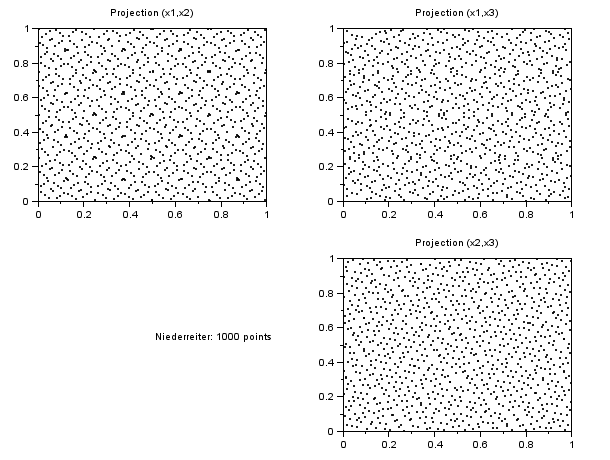
\includegraphics[width=15cm]{figures/niederreiter-s3-n1000.png}
\end{center}
\caption{Niederreiter sequence in base 2 - 1000 points in 3 dimensions.}
\label{fig-niederreiter-s3-n1000}
\end{figure}

\begin{figure}[htbp]
\begin{center}
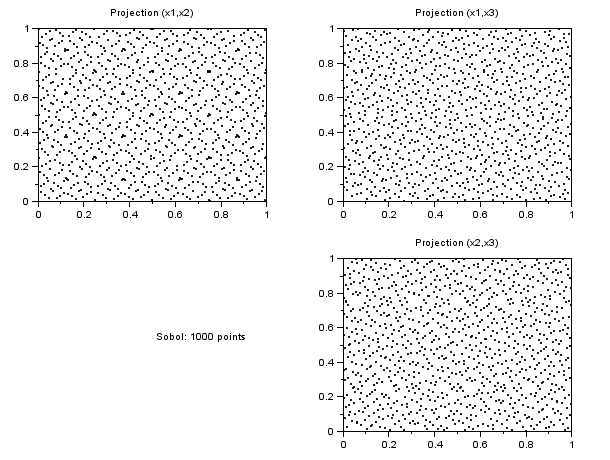
\includegraphics[width=15cm]{figures/sobol-s3-n1000.png}
\end{center}
\caption{Sobol sequence - 1000 points in 3 dimensions.}
\label{fig-sobol-s3-n1000}
\end{figure}

\begin{figure}[htbp]
\begin{center}
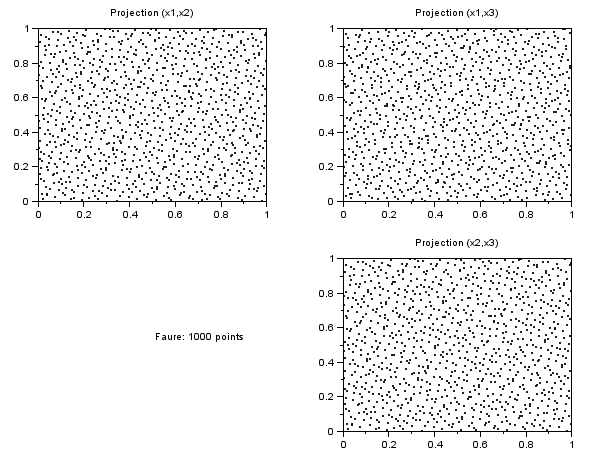
\includegraphics[width=15cm]{figures/faure-s3-n1000.png}
\end{center}
\caption{Faure sequence - 1000 points in 3 dimensions.}
\label{fig-faure-s3-n1000}
\end{figure}


    
      We see that the projection (x1,x2) is the same for 
	  Sobol and Niederreiter (base 2), as was seen for 2D sequences. 
	  But, the projections (x1,x3) and (x2,x3) of Sobol and Niederreiter 
	  are different. 
	  Moreover, all projections of Faure sequence are now different from the 
	  other sequences. 
	  Furthermore, the projection (x1,x2) of Faure is different from the 
	  Faure 2D sequence.
    
	
    
	  Indeed, the Faure sequence uses a basis which is the smallest prime number 
	  larger than the number of dimensions. 
	  In dimension s=3, the basis used by Faure is p=3. 
	  Since Sobol and Niederreiter (base 2) use the base 2, this explains 
	  why the sequences cannot be equal anymore.
 